%=================================================================
\chapter{CONTEXTO} \label{cha:background}
%=================================================================

En este cap\'itulo se realiza una revisi\'on de los conceptos empleados durante el desarrollo de este documento. 

%**************************************************************
\section{Alineaci\'on de Negocio-IT} \label{sec:bitalignment}
%**************************************************************
La alineaci\'on entre negocio y tecnolog\'ia puede ser definida como la forma de cuantificar el nivel de coherencia entre las necesidades del negocio y la respuesta ofrecida por las Tecnolog\'ias de Informaci\'on (IT) \cite{Pereira:2003}. Henderson y Venkatraman \cite{henderson:1990} definen el alineamiento estrat\'egico a partir de cuatro componentes: i) Estrateg\'ia de Negocio, ii) estrateg\'ia de IT, iii) procesos e infraestructura organizacional, y iv) procesos e infraestructura de IT. Las diferentes relaciones que se dan entre estos componentes son definidas como \textit{Alineamiento Estrat\'egico}, \textit{Alineamiento Funcional} y \textit{Alineamiento Transversal}.

Otros trabajos \cite{Pereira:2005, Wang:2008, Wang:20082, Plazaola:2008} han abordado la gesti\'on y evaluaci\'on del alineamiento en t\'erminos de los componentes contenidos en la EA. En la misma l\'inea, para el framework SEAM \cite{Wegmann:2005} el alineamiento negocio-IT corresponde a la trazabilidad entre los niveles de negocio, operaci\'on e IT. 

%**************************************************************
\section{Arquitectura Empresarial} \label{sec:eamda}
%**************************************************************

Una Arquitectura Empresarial (EA) ofrece la descripci\'on integral y estructurada de la organizaci\'on, sus Sistemas de Informaci\'on (IS), y la forma en que estos se integran a fin de alcanzar los objetivos de negocio apoyados en Tecnolog\'ias de Informaci\'on (IT). Esta descripci\'on se compone de documentos, diagramas y dem\'as artefactos que formalizan diferentes puntos de vista de la organizaci\'on, de tal manera que sean un referente y soporte para la toma de decisiones. Los frameworks tradicionales de EA como \cite{Zachman:1987, DoDAF:2005, OpenGroup:2008}, tienen en com\'un la desagregaci\'on en dimensiones: i) La \textit{Arquitectura de Negocio} (BA) define la estrategia, gobernabilidad, organizaci\'on y procesos claves de negocio. ii) La \textit{Arquitectura de Datos} (IA) describe la estructura de los activos de datos l\'ogicos y f\'isicos de la organizaci\'on y los recursos de gesti\'on de datos. iii) La \textit{Arquitectura de Aplicaciones} provee un modelo para las aplicaciones a ser desplegadas, sus interacciones y sus relaciones con los principales procesos de negocio de la organizaci\'on. iv) En la \textit{Arquitectura de Tecnolog\'ia} se describen las capacidades de software y hardware que son requeridas para el despliegue de servicios de negocio, datos y aplicaciones.

%===============================================================
\section{Arquitectura Dirigida por Modelos} \label{subsec:mda}
%===============================================================

Model-Driven Architecture (MDA) es una propuesta de la OMG para abordar el desarrollo de software proporcionando un conjunto de gu\'ias para estructurar especificaciones expresadas en modelos. Es neutral en cuanto a tecnolog\'ia y proveedor, y busca reducir significativamente el esfuerzo de desarrollo, separando la arquitectura del sistema, de las arquitecturas de plataforma. Uno de los elementos claves de MDA es el Modelo de Plataforma Independiente (\textit{PIM}) que describe la estructura y el comportamiento de un sistema, pero no su implementaci\'on. La implementanci\'on en la plataforma particular (JEE, .NET, WS, etc) est\'a definida en un Modelo de Plataforma Espec\'ifica (\textit{PSM}), el cual es originado a partir del PIM. Para materializar esta conversi\'on, se realizan transformaciones basadas en plantillas detalladas para cada plataforma, que mapean elementos del PIM hacia elementos PSM.

%===============================================================
\section{Tartarus} \label{subsec:tartarus}
%===============================================================


Tartarus es un acercamiento MDA para el an\'alisis de EAs \cite{Moosas:2011}. Tartarus surge como una opci\'on de soluci\'on ante la actual variedad de frameworks, est\'andares, herramientas y formatos que hacen parte de la definci\'on de una EA \cite{Rodriguez:2011}. El metamodelo descrito en la Figura \ref{fig:Tartarus-MM} est\'a compuesto por cinco paquetes: \textit{Enterprise} contiene la estructura, cadena de valor, principios, incentivos organizacionales y dem\'as elementos estrat\'egicos. \textit{Continuum} re\'une las definiciones para describir la manera en que la EA evoluciona. \textit{Management} tiene los factores necesarios para evaluar los artefactos que conforman una arquitectura. \textit{Environment} comprende el conjunto de elementos que describen el entorno en el que funciona la empresa. 

%........................................................
\begin{figure}[!t]
\begin{center}
	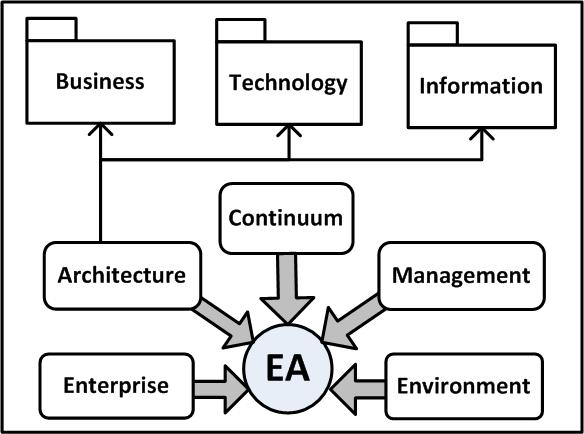
\includegraphics[scale=0.8 ,natwidth=584pt, natheight=434pt]{TartarusMM.jpg}
	\caption{Vista General del Metamodelo Tartarus}
	\label{fig:Tartarus-MM}
\end{center}
\end{figure}
%........................................................

\textit{Architecture} agrupa los conceptos clave para visualizar y estructurar la EA. \textit{Architecture} contiene los cuatro dominios: \textit{Business Domain}: Describe los procesos de negocio. \textit{Technology Domain}: Comprende las capacidades de software y hardware que soportan los servicios de negocio e informaci\'on. \textit{Information Domain}: Estructura los componentes de datos que conforman la informaci\'on de la empresa.

Vamos a describir el metamodelo, detallando el dominio de informaci\'on (izquierda), procesos de negocio (derecha) como parte del contexto de nuestro trabajo. La Figura \ref{fig:BA-IA-MM} muestra el metamodelo de los dominios mencionados.

%........................................................
\begin{landscape}

\begin{figure}[!t]
\begin{center}
	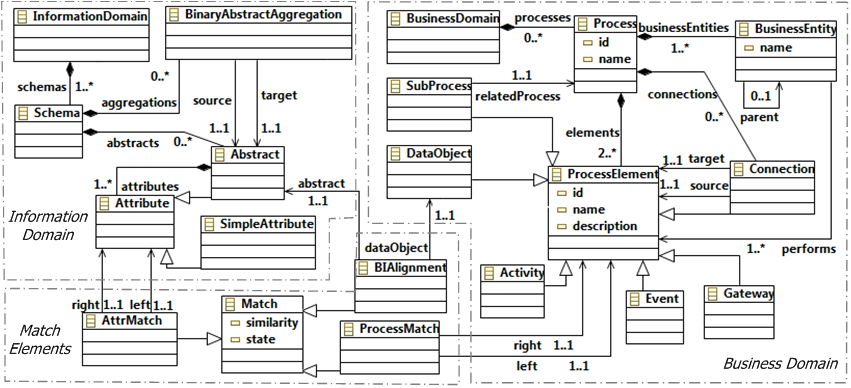
\includegraphics[scale=1 ,natwidth=851pt, natheight=388pt]{IA-BA_MM.png}
	\caption{Detalle del Metamodelo Tartarus y las Extensions  Kalcas}
	\label{fig:BA-IA-MM}
\end{center}
\end{figure}

\end{landscape}
%........................................................


%===============================================================
\subsection{Arquitectura de Negocio (BA)}
%===============================================================

Este dominio define los procesos de negocio de la compa\~n\'ia. En el metamodelo se resaltan los elementos de proceso (\texttt{ProcessElements}), Entidades de Negocio, Objetos de Flujo y Conexiones. El metamodelo aborda los diferentes tipos de actividades, eventos y flujos derivados de la nomenclatura BPMN (Business Process Modeling Notation). El concepto \texttt{DataObject} asocia las entidades de datos le\'idas y/o producidas por las actividades.

Para nuestro caso el Proceso de Registro corresponde a un elemento \texttt{Process} el cual contiene las once actividades (\texttt{Activity}) conectadas por elementos de clase \texttt{Connection} y/o \texttt{Gateway}. Los objetos de datos como \texttt{Payment Format} y \texttt{Card} se consignan como instancias de tipo \texttt{DataObject}.


%===============================================================
\subsection{Arquitectura de Informaci\'on (IA)}
%===============================================================

Nuestro metamodelo de arquitectura de informaci\'on es una adaptaci\'on del trabajo propuesto en \cite{Atzeni:2008}, enriquecido con las definiciones de las relaciones inferidas entre entidades, comentarios de tablas y comentarios de columnas. La metaclase \texttt{Schema} representa los esquemas contenidos en la EA. Para nuestro caso, el esquema \texttt{S1} se convierte en la instancia \texttt{Schema:S1}. La metaclase \texttt{Attribute} est\'a especializada en dos subclases: \texttt{SimpleAttribute} la cual define columnas en la base de datos o tipos primitivos en esquemas XML, tienen un tipo de dato (\texttt{INTEGER, DOUBLE, STRING}, etc). Por otro lado, \texttt{Abstract} se refiere a entidades en un modelo relacional o tipos de dato complejos en XML Schema.

Por ejemplo, la entidad \texttt{USER} del esquema \texttt{S1} se convierte en un objeto \texttt{Abstract:S1.USER} y cada uno de sus campos (\texttt{name, document}, etc) son objetos de clase \texttt{SimpleAttribute} con sus respectivos tipos de dato. En \texttt{BinaryAbstractAggregation}, se definen las relaciones existentes entre cada par de elementos \texttt{Abstract}. La relaci\'on entre las entidades \texttt{USER} e \texttt{REGISTRATION} se representa con la asociaci\'on \texttt{BinaryAbstractAggregation: USER\_REGISTRATION}. 


%===============================================================
\section{Ontolog\'ias} \label{subsec:ontology}
%===============================================================

Una ontolog\'ia, b\'asicamente, es una descripci\'on expl\'icita de un dominio de conocimiento espec\'ifico, definida en t\'erminos de sus conceptos, propiedades, atributos, restricciones e individuos \cite{Noy:2001}. Formalmente podemos definir una ontolog\'ia como: $O = \lbrace C, P, H^{C}, H^{P}, A^{O}, I, R^{I} \rbrace$. Donde $C$ es el conjunto de conceptos, $P$ el conjunto de propiedades. $H^{C}$ es la jerarqu\'ia de relaciones entre los conceptos tal que $H^{C} \subset C \times C (c_{i},c_{j}) \in H^{C}$ denota que el concepto $c_{i}$ es subconcepto de $c_{j}$. De la misma manera $H^{P}$ define las relaciones jer\'arquicas entre propiedades. $A^{O}$ es el conjunto de axiomas. I comprende el conjunto de Individuos, es decir, instancias de conceptos y propiedades quienes se asocian a trav\'es de instancias relacionales $R^{I}$. Una de las principales ventajas de las ontolog\'ias, es proveer caracter\'isticas \'utiles para sistemas inteligentes, representaci\'on e ingenier\'ia de conocimiento \cite{Gasevic:2009}.

%===============================================================
\subsection{Matching de Ontolog\'ias} \label{subsec:matching}
%===============================================================

La funci\'on de alineaci\'on de ontolo\'ias ha sido definida formalmente \cite{Euzenat:2007, Gal:2009}: $f(O_{1},O_{2}) = \lbrace e_{i1}, e_{i2}, i_{i}, r_{i}\rbrace$. Donde $O_{1}$ y $O_{2}$ son los esquemas/ontolog\'ias de entrada, com\'unmente llamados origen y destino respectivamente, $e_{i1}$ y $e_{i2}$ son las dos entidades comparadas, $i_{i}$ corresponde al \'indice de similitud o confianza (medido entre 0 y 1) y $r_{i}$ la relaci\'on (igualdad, especializaci\'on, generalizaci\'on) que puede haber entre $e_{i1}$ y $e_{i2}$. Detectar elementos similares entre diferentes fuentes de informaci\'on es tambi\'en una necesidad central en procesos de evaluaci\'on, migraci\'on, integraci\'on y evoluci\'on de SI, intercambio de informaci\'on en sistemas P2P y composici\'on de web services \cite{Euzenat:2007}.

En 2004 surge la Ontology Alignment Evaluation Initiative (\textit{OAEI}), una iniciativa que anualmente eval\'ua sistemas de alineamiento de ontolog\'ias. El objetivo de la OAEI es comparar diferentes propuestas, con el objetivo de ofrecer conclusiones sobre las mejores t\'ecnicas y estrategias, para lo cual, provee unos casos de prueba sobre los cuales los diferentes sistemas experimentan.  Entre los temas evaluados se encuentran: \textit{The benchmark track, The directories and thesauri track, Instance matching}. 

Existen diferentes m\'etodos y t\'ecnicas para implementar alineamiento autom\'atico de ontolog\'ias \cite{Madhavan:2001, Rahm:2001, Shvaiko:2005} y nuestra propuesta incluye algunos de ellos. Las principales t\'ecnicas de alineamiento son \textit{basadas en esquema}, \textit{basadas en contenido} y \textit{combinadas}. Las \textit{basadas en esquema} s\'olo tienen en cuenta la informaci\'on estructural del esquema, no su contenido. Dentro de este grupo se aplican comparaciones ling\"u\'isticas, textuales, de restricciones y estructurales. Las estrategias \textit{basadas en contenido} involucran estad\'isticas, patrones o incluso los mismos datos para inferir correspondencias. Las t\'ecnicas \textit{combinadas} aplican, en conjunto, las anteriores aproximaciones en busca de mejores resultados. Esta combinaci\'on puede ser configurada manual o autom\'aticamente utilizando aprendizaje de m\'aquina. 

Este trabajo no busca determinar la mejor forma de realizar alineamientos, sino adaptar y aplicar t\'ecnicas y avances en el \'area de matching de ontolog\'ias para inferir trazabilidad entre componentes de procesos e informaci\'on.